%% abtex2-modelo-trabalho-academico.tex, laurocesar
%% Copyright 2012-2015 by abnTeX2 group at http://www.abntex.net.br/ 
%%
%% This work may be distributed and/or modified under the
%% conditions of the LaTeX Project Public License, either version 1.3
%% of this license or (at your option) any later version.
%% The latest version of this license is in
%%   http://www.latex-project.org/lppl.txt
%% and version 1.3 or later is part of all distributions of LaTeX
%% version 2005/12/01 or later.
%%
%% This work has the LPPL maintenance status `maintained'.
%% 
%% The Current Maintainer of this work is the abnTeX2 team, led
%% by Lauro César Araujo. Further information are available on 
%% http://www.abntex.net.br/
%%
%% This work consists of the files abntex2-modelo-trabalho-academico.tex,
%% abntex2-modelo-include-comandos and abntex2-modelo-references.bib
%%

% ------------------------------------------------------------------------
% ------------------------------------------------------------------------
% abnTeX2: Modelo de Trabalho Academico (tese de doutorado, dissertacao de
% mestrado e trabalhos monograficos em geral) em conformidade com 
% ABNT NBR 14724:2011: Informacao e documentacao - Trabalhos academicos -
% Apresentacao
% ------------------------------------------------------------------------
% ------------------------------------------------------------------------

\documentclass[
	% -- opções da classe memoir --
	12pt,				% tamanho da fonte
	openright,			% capítulos começam em pág ímpar (insere página vazia caso preciso)
	oneside,			% para impressão em verso e anverso. Oposto a oneside
	a4paper,			% tamanho do papel. 
	% -- opções da classe abntex2 --
	chapter=TITLE,		% títulos de capítulos convertidos em letras maiúsculas
	%section=TITLE,		% títulos de seções convertidos em letras maiúsculas
	%subsection=TITLE,	% títulos de subseções convertidos em letras maiúsculas
	%subsubsection=TITLE,% títulos de subsubseções convertidos em letras maiúsculas
	% -- opções do pacote babel --
	english,			% idioma adicional para hifenização
	french,				% idioma adicional para hifenização
	spanish,			% idioma adicional para hifenização
	brazil				% o último idioma é o principal do documento
	]{abntex2}

% ---
% Pacotes básicos 
% ---
\usepackage{helvet}			% Usa a fonte Latin Modern - Mudei para Helvetica
\usepackage[T1]{fontenc}		% Selecao de codigos de fonte.
\usepackage[utf8]{inputenc}	% Codificacao do documento (conversão automática dos acentos)
\usepackage{lastpage}		% Usado pela Ficha catalográfica
\usepackage{indentfirst}		% Indenta o primeiro parágrafo de cada seção.
\usepackage{color}			% Controle das cores
\usepackage{graphicx}		% Inclusão de gráficos
\usepackage{microtype} 		% para melhorias de justificação
% ---
		
% ---
% Pacotes adicionais, usados apenas no âmbito do Modelo Canônico do abnteX2
% ---
\usepackage{lipsum}				% para geração de dummy text
\usepackage{customizacoes} 		% customizações feitas pelo autor
% ---

% ---
% Pacotes de citações
% ---
\usepackage[brazilian,hyperpageref]{backref}	% Paginas com as citações na bibl
\usepackage[alf]{abntex2cite}				% Citações padrão ABNT

% --- 
% CONFIGURAÇÕES DE PACOTES
% --- 

% ---
% Configurações do pacote backref
% Usado sem a opção hyperpageref de backref
\renewcommand{\backrefpagesname}{ }
% Texto padrão antes do número das páginas
\renewcommand{\backref}{\ABNTEXchapterfont}
% Define os textos da citação
\renewcommand*{\backrefalt}[4]{
	\ifcase #1 %
		%
	\or
		%
	\else
		%
	\fi}%
% ---

% ---
% Informações de dados para CAPA e FOLHA DE ROSTO
% ---
\titulo{Desenvolvimento de um Protótipo de Rastreador de Beacons utilizando o Raspberry Pi}
\autor{Gabriel Luiz Bastos Oliveira}
\local{Bauru}
\data{2015}
\orientador{Prof. Dr. Eduardo Martins Morgado}
\instituicao{%
  Universidade Estadual Paulista "Júlio de Mesquita Filho"
  \par
  Faculdade de Ciências - Campus Bauru
  \par
  Departamento de Computação
}
\tipotrabalho{Monografia (Trabalho de Conclusão de Curso)}
% O preambulo deve conter o tipo do trabalho, o objetivo, 
% o nome da instituição e a área de concentração 
\preambulo{Anteprojeto de pesquisa apresentado como requisito da disciplina de Projeto de Implementação de Sistemas I do curso de Ciência da Computação.}
% ---

% ---
% Configurações de projeto
% --- 
\newif\iffinal
\finalfalse % define se é um arquivo final, se for não for retira umas partes. 

\newif\ifabstract
\abstractfalse % define se mostra o abstract em inglês ou não.

% --- 


% ---
% Configurações de aparência do PDF final

% alterando o aspecto da cor azul
\definecolor{blue}{RGB}{0,0,0}

% informações do PDF
\makeatletter
\hypersetup{
     	%pagebackref=true,
		pdftitle={\@title}, 
		pdfauthor={\@author},
    	pdfsubject={\imprimirpreambulo},
	    pdfcreator={LaTeX with abnTeX2},
		pdfkeywords={beacon}{raspberry pi}{internet das coisas}{abntex2}{trabalho acadêmico}, 
		colorlinks=true,       		% false: boxed links; true: colored links
    	linkcolor=blue,          	% color of internal links
    	citecolor=blue,        		% color of links to bibliography
    	filecolor=magenta,      		% color of file links
		urlcolor=blue,
		bookmarksdepth=4
}
\makeatother
% --- 

% --- 
% Espaçamentos entre linhas e parágrafos 
% --- 

% O tamanho do parágrafo é dado por:
\setlength{\parindent}{1.3cm}

% Controle do espaçamento entre um parágrafo e outro:
\setlength{\parskip}{0.2cm}  % tente também \onelineskip

% ---
% compila o indice
% ---
\makeindex
% ---

% ----
% Início do documento
% ----
\begin{document}

% Seleciona o idioma do documento (conforme pacotes do babel)
%\selectlanguage{english}
\selectlanguage{brazil}

% Retira espaço extra obsoleto entre as frases.
\frenchspacing 

% ----------------------------------------------------------
% ELEMENTOS PRÉ-TEXTUAIS
% ----------------------------------------------------------
\pretextual

\ABNTEXchapterfont {

% ---
% Capa
% ---
\imprimircapa
% ---

% ---
% Folha de rosto
% (o * indica que haverá a ficha bibliográfica)
% ---
\imprimirfolhaderosto
% ---

% ---
% Inserir a ficha bibliografica
% ---

% Isto é um exemplo de Ficha Catalográfica, ou ``Dados internacionais de
% catalogação-na-publicação''. Você pode utilizar este modelo como referência. 
% Porém, provavelmente a biblioteca da sua universidade lhe fornecerá um PDF
% com a ficha catalográfica definitiva após a defesa do trabalho. Quando estiver
% com o documento, salve-o como PDF no diretório do seu projeto e substitua todo
% o conteúdo de implementação deste arquivo pelo comando abaixo:
%
% \begin{fichacatalografica}
%     \includepdf{fig_ficha_catalografica.pdf}
% \end{fichacatalografica}

\iffinal
  \begin{fichacatalografica}
	\sffamily
	\vspace*{\fill}					% Posição vertical
	\begin{center}					% Minipage Centralizado
	\fbox{\begin{minipage}[c][8cm]{13.5cm}		% Largura
	\small
	\imprimirautor
	%Sobrenome, Nome do autor
	
	\hspace{0.5cm} \imprimirtitulo  / \imprimirautor. --
	\imprimirlocal, \imprimirdata-
	
	\hspace{0.5cm} \pageref{LastPage} p. : il. (algumas color.) ; 30 cm.\\
	
	\hspace{0.5cm} \imprimirorientadorRotulo~\imprimirorientador\\
	
	\hspace{0.5cm}
	\parbox[t]{\textwidth}{\imprimirtipotrabalho~--~\\ \imprimirinstituicao,
	\imprimirdata.}\\
	
	\hspace{0.5cm}
		1. Beacon.
		2. Raspberry Pi.
		2. Internet das Coisas.
		I. \imprimirorientador.
		II. Universidade Estadual Paulista "Júlio de Mesquita Filho".
		III. Faculdade de Ciências.
		IV. Título
	\end{minipage}}
	\end{center}
  \end{fichacatalografica}
\fi
% ---

% ---
% Inserir errata
% ---
%\begin{errata}
%Elemento opcional da \citeonline[4.2.1.2]{NBR14724:2011}. Exemplo:

%\vspace{\onelineskip}

%FERRIGNO, C. R. A. \textbf{Tratamento de neoplasias ósseas apendiculares com
%reimplantação de enxerto ósseo autólogo autoclavado associado ao plasma
%rico em plaquetas}: estudo crítico na cirurgia de preservação de membro em
%cães. 2011. 128 f. Tese (Livre-Docência) - Faculdade de Medicina Veterinária e
%Zootecnia, Universidade de São Paulo, São Paulo, 2011.

%\begin{table}[htb]
%\center
%\footnotesize
%\begin{tabular}{|p{1.4cm}|p{1cm}|p{3cm}|p{3cm}|}
%  \hline
%   \textbf{Folha} & \textbf{Linha}  & \textbf{Onde se lê}  & \textbf{Leia-se}  \\
%    \hline
%    1 & 10 & auto-conclavo & autoconclavo\\
%   \hline
%\end{tabular}
%\end{table}

%\end{errata}
% ---

% ---
% Inserir folha de aprovação
% ---

% Isto é um exemplo de Folha de aprovação, elemento obrigatório da NBR
% 14724/2011 (seção 4.2.1.3). Você pode utilizar este modelo até a aprovação
% do trabalho. Após isso, substitua todo o conteúdo deste arquivo por uma
% imagem da página assinada pela banca com o comando abaixo:
%
% \includepdf{folhadeaprovacao_final.pdf}
%
\begin{folhadeaprovacao}
  \ABNTEXchapterfont {

    \begin{center}
    
      {\ImprimirAutor}

      \vspace*{\fill}\vspace*{\fill}
      
      \begin{center}
        \bfseries\large\ImprimirTitulo
      \end{center}
      
      \vspace*{\fill}
    
      \hspace{.45\textwidth}
      \begin{minipage}{.5\textwidth}
          \imprimirpreambulo
      \end{minipage}%
      \vspace*{\fill}
     \end{center}
        
     %Trabalho aprovado. \imprimirlocal, 24 de novembro de 2012:

     \assinatura{\textbf{\imprimirorientador} \\ Orientador} 
     %\assinatura{\textbf{Professor} \\ Convidado 1}
     %\assinatura{\textbf{Professor} \\ Convidado 2}
     %\assinatura{\textbf{Professor} \\ Convidado 3}
     %\assinatura{\textbf{Professor} \\ Convidado 4}
      \vspace*{0.5cm}
      \hspace{.5\textwidth}
     \begin{center} 
       \ImprimirLocal \\ \imprimirdata
     \end{center}
  }
\end{folhadeaprovacao}
% ---

% ---
% Dedicatória
% ---
\iffinal
  \begin{dedicatoria} 
   \vspace*{\fill}
   \centering
   \noindent
   \textit{ Este trabalho é dedicado às crianças adultas que,\\
   quando pequenas, sonharam em se tornar cientistas.} \vspace*{\fill}
  \end{dedicatoria}
\fi
% ---

% ---
% Agradecimentos
% ---
\iffinal
  \begin{agradecimentos}
Os agradecimentos principais são direcionados à Gerald Weber, Miguel Frasson,
Leslie H. Watter, Bruno Parente Lima, Flávio de Vasconcellos Corrêa, Otavio Real
Salvador, Renato Machnievscz\footnote{Os nomes dos integrantes do primeiro
projeto abn\TeX\ foram extraídos de
\url{http://codigolivre.org.br/projects/abntex/}} e todos aqueles que
contribuíram para que a produção de trabalhos acadêmicos conforme
as normas ABNT com \LaTeX\ fosse possível.

Agradecimentos especiais são direcionados ao Centro de Pesquisa em Arquitetura
da Informação\footnote{\url{http://www.cpai.unb.br/}} da Universidade de
Brasília (CPAI), ao grupo de usuários
\emph{latex-br}\footnote{\url{http://groups.google.com/group/latex-br}} e aos
novos voluntários do grupo
\emph{\abnTeX}\footnote{\url{http://groups.google.com/group/abntex2} e
\url{http://www.abntex.net.br/}}~que contribuíram e que ainda
contribuirão para a evolução do \abnTeX.

\end{agradecimentos}
\fi
% ---

% ---
% Epígrafe
% ---
\iffinal
  \begin{epigrafe}
    \vspace*{\fill}
	\begin{flushright}
		\textit{``Não vos amoldeis às estruturas deste mundo, \\
		mas transformai-vos pela renovação da mente, \\
		a fim de distinguir qual é a vontade de Deus: \\
		o que é bom, o que Lhe é agradável, o que é perfeito.\\
		(Bíblia Sagrada, Romanos 12, 2)}
	\end{flushright}
  \end{epigrafe}
\fi
% ---

% ---
% RESUMOS
% ---
\ifabstract
% resumo em português
\setlength{\absparsep}{18pt} % ajusta o espaçamento dos parágrafos do resumo
\begin{resumo}
\ABNTEXchapterfont {
 Segundo a , o resumo deve ressaltar o
 objetivo, o método, os resultados e as conclusões do documento. A ordem e a extensão
 destes itens dependem do tipo de resumo (informativo ou indicativo) e do
 tratamento que cada item recebe no documento original. O resumo deve ser
 precedido da referência do documento, com exceção do resumo inserido no
 próprio documento. (\ldots) As palavras-chave devem figurar logo abaixo do
 resumo, antecedidas da expressão Palavras-chave:, separadas entre si por
 ponto e finalizadas também por ponto.

 \textbf{Palavras-chave}: \textit{Beacon}. Raspberry Pi. Internet das Coisas.
}
\end{resumo}

% resumo em inglês
\begin{resumo}[Abstract]
 \begin{otherlanguage*}{english}
   This is the english abstract.

   \vspace{\onelineskip}
 
   \noindent 
   \textbf{Keywords}: Beacon. Raspberry Pi. Internet of Things.
 \end{otherlanguage*}
\end{resumo}
\fi
% ---

% ---
% inserir lista de ilustrações
% ---
\iffinal
  \pdfbookmark[0]{\listfigurename}{lof}
  \listoffigures*
  \cleardoublepage
\fi
% ---

% ---
% inserir lista de tabelas
% ---
\iffinal
  \pdfbookmark[0]{\listtablename}{lot}
  \listoftables*
  \cleardoublepage
\fi
% ---

% ---
% inserir lista de abreviaturas e siglas
% ---
\iffinal
  \begin{siglas}
    \item[IoT] \textit{Internet of Things}
    \item[DIY] \textit{Do It Yourself}
    \item[GPIO] \textit{General Input and Output}
    \item[BLE] \textit{Bluetooth Low Energy}
  \end{siglas}
\fi
% ---

% ---
% inserir lista de símbolos
% ---
\iffinal
  \begin{simbolos}
    \item[$ \Gamma $] Letra grega Gama
    \item[$ \Lambda $] Lambda
    \item[$ \zeta $] Letra grega minúscula zeta
    \item[$ \in $] Pertence
  \end{simbolos}
\fi
% ---

% ---
% inserir o sumario
% ---
\pdfbookmark[0]{\contentsname}{toc}
\tableofcontents*
\cleardoublepage
% ---






% ----------------------------------------------------------------------------------------------------------------------------------
% ELEMENTOS TEXTUAIS
% ----------------------------------------------------------------------------------------------------------------------------------
\textual

% ---
% Introdução
% ---
\chapter[Introdução]{Introdução}
%\addcontentsline{toc}{chapter}{Introdução}
% ----------------------------------------------------------

A internet cresce dia após dia e cada vez mais diferentes tipos de dispositivos são conectados a essa imensa rede. Há uma estimativa de 26 bilhões de ''coisas'' conectadas a internet até 2020, comparado a 6 bilhões na década de 2000. Isso foi possível graças ao custo do acesso a internet e largura de banda (quantidade de dados trafegados) ter diminuído 40 vezes nos últimos 10 anos. Esse \textit{boom} de crescimento também é influenciado pela IoT (\textit{Internet of Things} - Internet das Coisas). \cite{goldmansachs-iot}. 

Segundo \citeonline{ashton-iot} o termo IoT surgiu como título de sua apresentação a Procter \& Gamble (P\&G) em 1999. Esse termo se dá ao uso de internet em diferentes tipos de dispositivos. 

\begin{citacao}
''(...) a Internet das Coisas é um conceito no qual dispositivos de nosso dia a dia são equipados com sensores capazes de captar aspectos do mundo real, como por exemplo, temperatura, umidade, presença, etc, e envia-los a centrais que recebem estas informações e as utilizam de forma inteligente.'' \cite{nascimento-iot}.
\end{citacao}

Como exemplo podemos citar: geladeira ligada a internet informando a falta de condimentos, caixa de remédio conectada a internet prevendo o término da caixa de remédio para avisar ao consumidor, entre diversos outros. Um bom exemplo é interligar uma casa por meio de sensores, como termostatos, sistemas de segurança, iluminação, sistemas de entretenimento com uma inteligência por trás para diversas aplicações. \cite{goldmansachs-iot}

Diversas áreas tiveram o seu crescimento alavancado por conta da IoT. O mais marcante é o ramo do DIY (\textit{Do It Yourself}, ou faça você mesmo), em que pessoas criam ou adaptam coisas para suas necessidades. Isso se dá por conta de ter aparecido no mercado dispositivos e componentes que auxiliam a criação e adaptação de eletrônicos e outros. Um ótimo exemplo é o Arduino, um dispositivo que nos ajuda a criar os projetos de eletrônica que consiste de duas partes: o hardware e o software. Com eles é possível construir praticamente de tudo, desde um LED piscante a um robô que envia um \textit{tweet} quando sua planta está sem água. \cite{ben-arduino}. \cite{sorrel-arduino}.

Além do Arduino existem diversos outros \textit{devices} com funcionalidades similares ou até complementares. Podemos citar o \textit{Raspberry Pi}, um computador do tamanho de um cartão de crédito e de baixo custo. \cite{raspberrypi-rpi}. Por ser um computador é possível executar um sistema operacional (como Linux, \textit{RISC OS}, \textit{Windows 10 for IoT}). Dependendo do modelo possui portas USB (1 a 4) para conexão com periféricos (como mouse, teclado, adaptador WiFi, Bluetooth), e também porta Ethernet para conexão a internet cabeada (exceto modelo A e A+). Também possui de 26 (modelo A e B) a 40 pinos (modelo A+, B+ e 2) para conexões gerais de entrada e saída digitais (GPIO - \textit{General Input and Output}). 

Através desses pinos pode-se conectar uma diversidade de componentes eletrônicos como sensores, atuadores, outros dispositivos para comunicação. Dessa forma, suas funcionalidades são expandidas de uma forma absurda, ficando a cargo de cada pessoa montar uma nova aplicação. Uma boa aplicação é a conexão de um adaptador bluetooth pela USB para comunicação com smartphones, tablets, PCs e outros dispositivos tipo sensores sem fio.

Um exemplo desses sensores externos são os \textit{beacons}, pequenos modelos sem fio que se comunicam por meio do Bluetooth 4.0 ou BLE (\textit{Bluetooth Low Energy} - Bluetooth de Baixa Energia). Como o próprio nome diz, esse padrão de comunicação utiliza muita pouca energia. Desta forma, um \textit{beacon} pode funcionar por anos. ''Na prática, ela permite localizar objetos (ou pessoas que carregam esses objetos) com muito mais precisão dentro de ambientes fechados.'' \cite{teixeira-beacon}.

% ---

% ---
% Problema
% ---
\chapter{Problema}
% ---

Os \textit{beacons} foram pouco explorados até o momento, seu uso está sendo mais notado na área de grandes lojas do varejo.

\begin{citacao}
''A Apple (...) já está utilizando a tecnologia em 254 lojas nos EUA. As funcionalidades já estão embutidas na versão oficial do aplicativo da Apple Store para iOS [, sistema operacional de seus smartphones e tablets]. (...) Quando o usuário se aproxima de uma loja física, o aplicativo oferece toda uma camada extra de informações e serviços que são específicos para aquela unidade – como por exemplo ofertas locais, tamanho da fila para ser atendido no Genius Bar, eventos e treinamentos que estão agendados ali na loja etc.'' \cite{teixeira-beacon}.
\end{citacao}

A Macy's (grande rede norte americana de loja de departamentos) está realizando testes em algumas de suas lojas para enviar alertas a pessoas que entrarem em suas lojas, com promoções e melhores indicações, utilizando o padrão \textit{iBeacon} da Apple. Até o momento esse teste está limitado a usuários de iPhone, e somente quando entrar na loja. Em um teste futuro espera-se que seja possível separar por departamentos, para que quando um usuário percorra a loja apareça as notícias relativo ao local da loja que ela está. \cite{kastrenakes-macys-beacon}

Porém as maiores aplicações são voltadas a smartphones e tablets como receptores e identificadores dos \textit{beacons}. Existem diversas empresas desenvolvendo variados tipos de \textit{beacons}, mas a maioria delas utiliza aplicativos para \textit{mobile devices} como identificadores. 

Alguns motivos podem ser apresentados para isso, mas o mais relevante é que até o momento poucas pessoas, grupos e empresas dedicaram tempo e dinheiro para investir nessa nova tecnologia. Um grande problema também é a necessidade de ter o \textit{bluetooth} ligado e permitindo conexões para que um smartphone consiga identificar os \textit{beacons}.

Esse projeto se propõe a desenvolver um protótipo utilizando outro meio para rastrear os \textit{beacons}, neste caso o \textit{Raspberry Pi}. Desta forma será possível explorar maiores aplicações aos \textit{beacons}.



% ---

% ---
% Justificativa
% ---
\chapter{Justificativa}
% ---

Os \textit{beacons} ainda estão em fase de descobrimento, não existem aplicações totalmente definidas e cada dia mais empresas investem nessa área. Pelas aplicações atuais serem totalmente voltadas a smartphones e tablets, a proposta desse projeto é tentar partir para uma área diferente e utilizar um outro dispositivo para realizar o descobrimento e rastreamento dos \textit{beacons}.

Como visto anteriormente, o \textit{Raspberry Pi} é um computador pequeno e de baixo custo, e também tem portas de entrada e saída digitais e portas USB. Por conta disso é possível expandir suas funcionalidades conectando módulos de \textit{bluetooth}, \textit{WiFi}, entre outros, podendo ser utilizado como um ótimo dispositivo de prototipagem.

Por ter uma comunidade grande e ativa, o seu estudo é facilitado. Um bom número de sites e comunidades estão desenvolvendo projetos com esse dispositivo e publicando suas conquistas. É possível encontrar tutoriais e passo-a-passo de um bom número de projetos, porém somente para aprendizado. Ao desenvolver um projeto mais elaborado isso pode servir como guia de estudo e aprofundamento.

As empresas tem investido um bom dinheiro na área de \textit{DIY} e \textit{IoT}. Existe uma grande expectativa para o futuro, por ser uma tecnologia barata para ser aplicada a grandes volumes, ter bastante gente envolvida e engajada, e também sua grande facilidade de criação.



% ---

% ---
% Objetivos
% ---
\chapter{Objetivos}
% ---

% ---

% ---
\section{Objetivos Gerais}
% ---

O objetivo geral desse projeto é planejar e desenvolver um protótipo de rastreador de \textit{beacons} utilizando o \textit{Raspberry Pi}.

% ---

% ---
\section{Objetivos Específicos}
% ---

\begin{alineas}
	\item Estudar o funcionamento de \textit{beacons}, comunicação via \textit{bluetooth low energy} e \textit{Raspberry Pi}, assim como suas aplicações.
	\item Identificar os requerimentos básicos de funcionamento de \textit{beacons} e \textit{Raspberry Pi}.
	\item Definir os elementos para desenvolvimento do protótipo.
	\item Planejar a estrutura do sistema.
	\item Implementar o protótipo de acordo com a estrutura e elementos planejados.
\end{alineas}

% ---

% ---
% Método de Pesquisa
% ---
\chapter{Método de Pesquisa}
% ---

O levantamento bibliográfico relacionado ao tema será a primeira fase dessa pesquisa, se buscará os assuntos relacionados a: \textit{Raspberry Pi}, comunicação via \textit{Bluetooth Low Energy}, \textit{beacons}. Concomitantemente será realizado o estudo das tecnologias, suas capacidades, limitações, aplicações, etc.

O segundo passo se planejará o projeto baseado na análise do levantamento bibliográfico, assim sua estrutura será definida. Essa etapa será necessária para facilitar e agilizar a implementação e testes dos componentes, definindo assim um escopo inicial de funcionalidades que o sistema deverá ter, assim como outras tarefas a serem realizadas.

Em seguida inicializará implementação e teste do protótipo. O projeto será desenvolvido por etapas, sendo que a primeira será o estudo de identificação dos \textit{beacons} via smartphone, a segunda o desenvolvimento software de identificação no \textit{Raspberry Pi}, e a terceira um aprimoramento do software embarcado para rastrear os \textit{beacons}. Em seguida serão realizados testes unitários experimentais em laboratório para que o protótipo possa ser aprimorado. Será testado com mais de um modelo de \textit{Raspberry Pi} e também mais de um \textit{beacon}, em ambiente aberto e fechado. Ao final espera-se ter um protótipo finalizado.

A etapa de testes será realizada por observação e experimentação nos ambientes. Os dados serão apresentados ao final do projeto pela confecção e apresentação da monografia.

% ---

% ---
% Fundamentação Teórica
% ---
\chapter{Fundamentação Teórica}
% ---

A área de IoT está em uma onda crescente, com um grande número de pessoas gastando nesse mercado, e um bom número de profissionais migrando para essa área. Há uma estimativa de que existem 19 milhões de profissionais trabalhando na indústria de desenvolvimento de software, e desses, 19\% trabalham em algum projeto relacionado a IoT. \cite{cw-iot}.

\begin{citacao}
''A próxima onda na era da computação será fora do domínio do ambiente de trabalho tradicional. No paradigma da IoT, muitos dos objetos que nos rodeiam estarão na rede de uma forma ou de outra. RFID (Radio Frequency Identification - Identificadores via Rádio Frequência) e as tecnologias de redes de sensores crescerão para enfrentar este novo desafio, em que os sistemas de informação e comunicação estão embutidos nos ambientes que nos rodeiam, de forma invisível.''. \cite{iot-article}. 
\end{citacao}

É notável o crescimento dessa área. Há uma expectativa de que, em 2020, o número de carros conectados a internet supere o número de carros não conectados, sendo esses carros possíveis de se comunicar com outros veículos e a infraestrutura das ruas, como os semáforos. \cite{goldmansachs-iot}. Segundo \citeonline{press-iot}, em 2014 a IoT substituiu a área da \textit{Big Data} como a tecnologia mais empolgante, ou seja, a tecnologia que mais pessoas iriam migrar e se interessar. 

Quando se pesquisa algo relacionado a IoT é praticamente impossível não achar relação e links para \textit{Raspberry Pi} (figura~\ref{fig:rpia-rpi2b}), Arduinos, e toda a área de \textit{DIY}. 


		\begin{figure}[h!]
			\ABNTEXchapterfont {
				\centering
				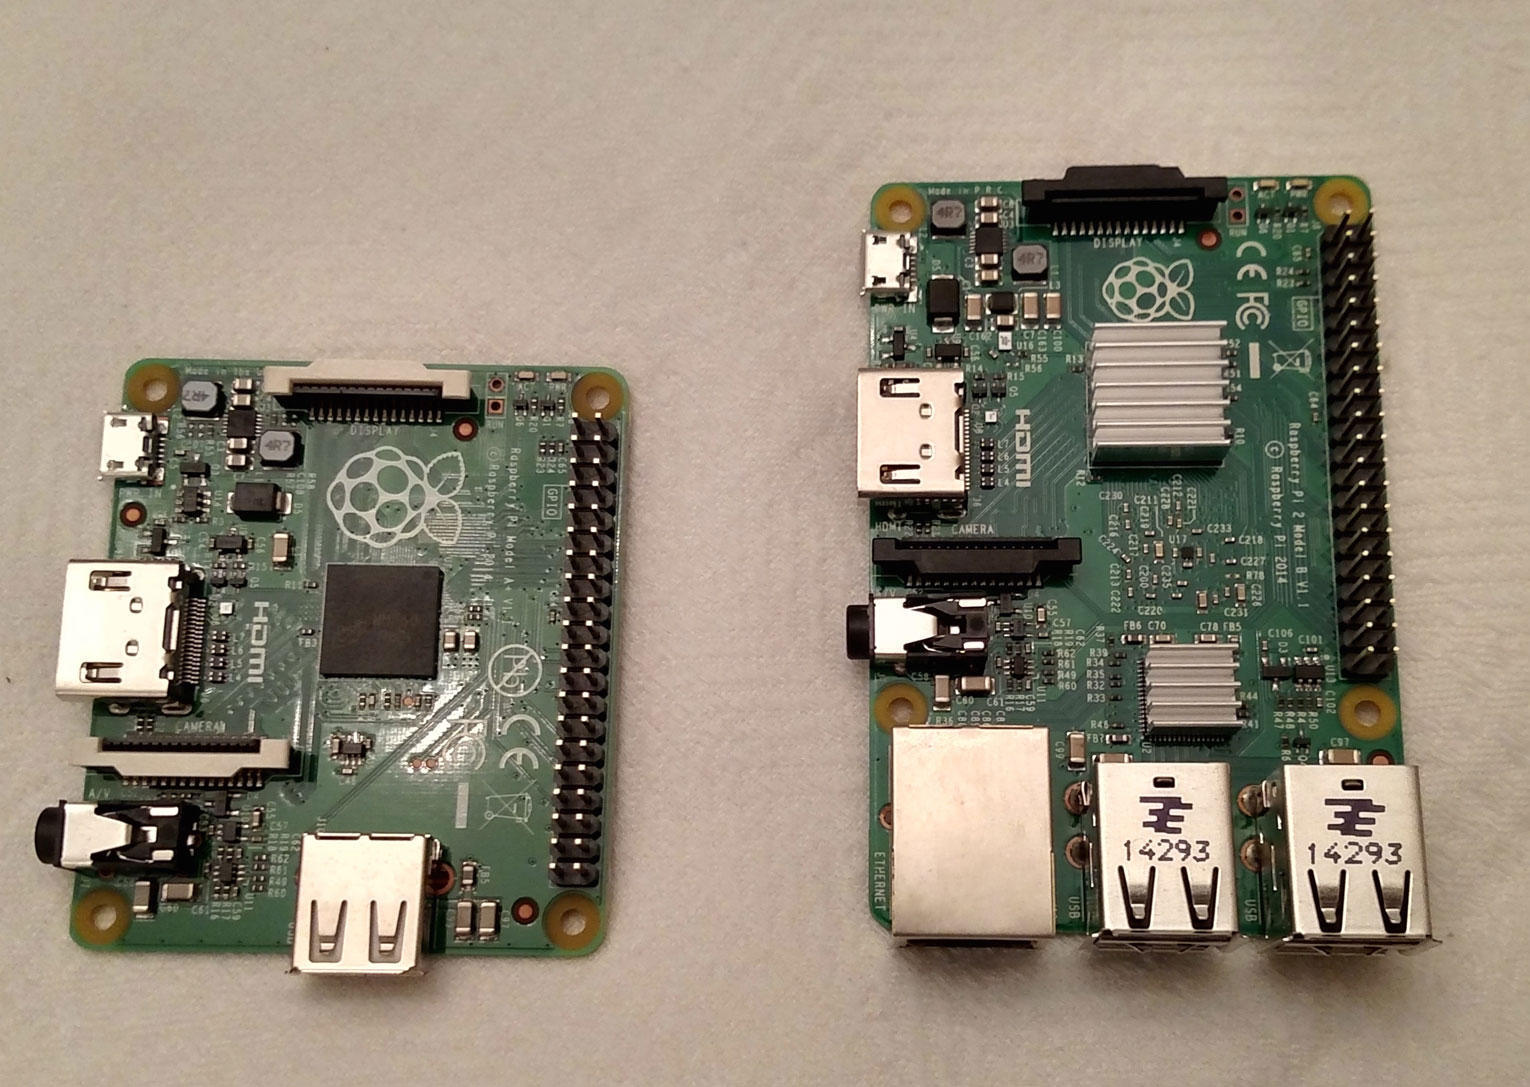
\includegraphics[width=0.6\textwidth]{img/rpia-rpi2b.jpg}
				\caption{\textit{Raspberry Pi} modelo A+ (esquerda) e \textit{Raspberry Pi} 2 modelo B (direita).}
				\label{fig:rpia-rpi2b}
			}
		\end{figure}

O \textit{Raspberry Pi} é um computador bem pequeno, demonstrado na figura~\ref{fig:rpia-rpi2b}. Segundo \citeonline{raspberrypi-rpi}, a fundação responsável pela criação desse pequeno dispositivo gostaria de ver ele ser usado por crianças e pessoas carentes do mundo todo para aprender a programar e como a computação funciona. É facilmente configurável, utilizando um cartão de memória como HD para salvar dados e o sistema operacional.

Por meio de suas portas de entrada e saída digitais é possível conectar uma gama ampla de sensores, atuadores, compontentes eletrônicos, ficando a cargo do programador e criador do projeto a escolher como esses pinos serão conectados e aproveitados. Atualmente existem diversos módulos para expandir os meios de comunicação entre diferentes \textit{devices}, e um deles é via \textit{bluetooth}.

A tecnologia do \textit{bluetooth} vem sendo amplamente utilizada, principalmente após a criação da versão 4.0, ou \textit{BLE} (\textit{Bluetooth Low Energy} - Bluetooth de Baixa Energia), por conta de ter um baixíssimo gasto energético, podendo preservar a bateria do dispositivo que a utiliza. Um ótimo exemplo são os \textit{beacons}, pequenos sensores que são capazes de identificar objetos com precisão dentro de ambientes fechados. \cite{teixeira-beacon}.

\begin{citacao}
Como muitos espaços fechados (restaurantes, museus, shopping centers, casas de show) possuem estrutura metálica ou utilizam algum tipo de metal em sua construção, é comum que o sinal de GPS fique enfraquecido quando os usuários estão dentro daquele local. Nesse caso, os \textit{Beacons} são uma ótima solução: um hardware relativamente barato, e pequeno o suficiente para ser plugado na parede ou instalado sobre um balcão. \cite{teixeira-beacon}.
\end{citacao}

		\begin{figure}[h!]
			\ABNTEXchapterfont {
				\centering
				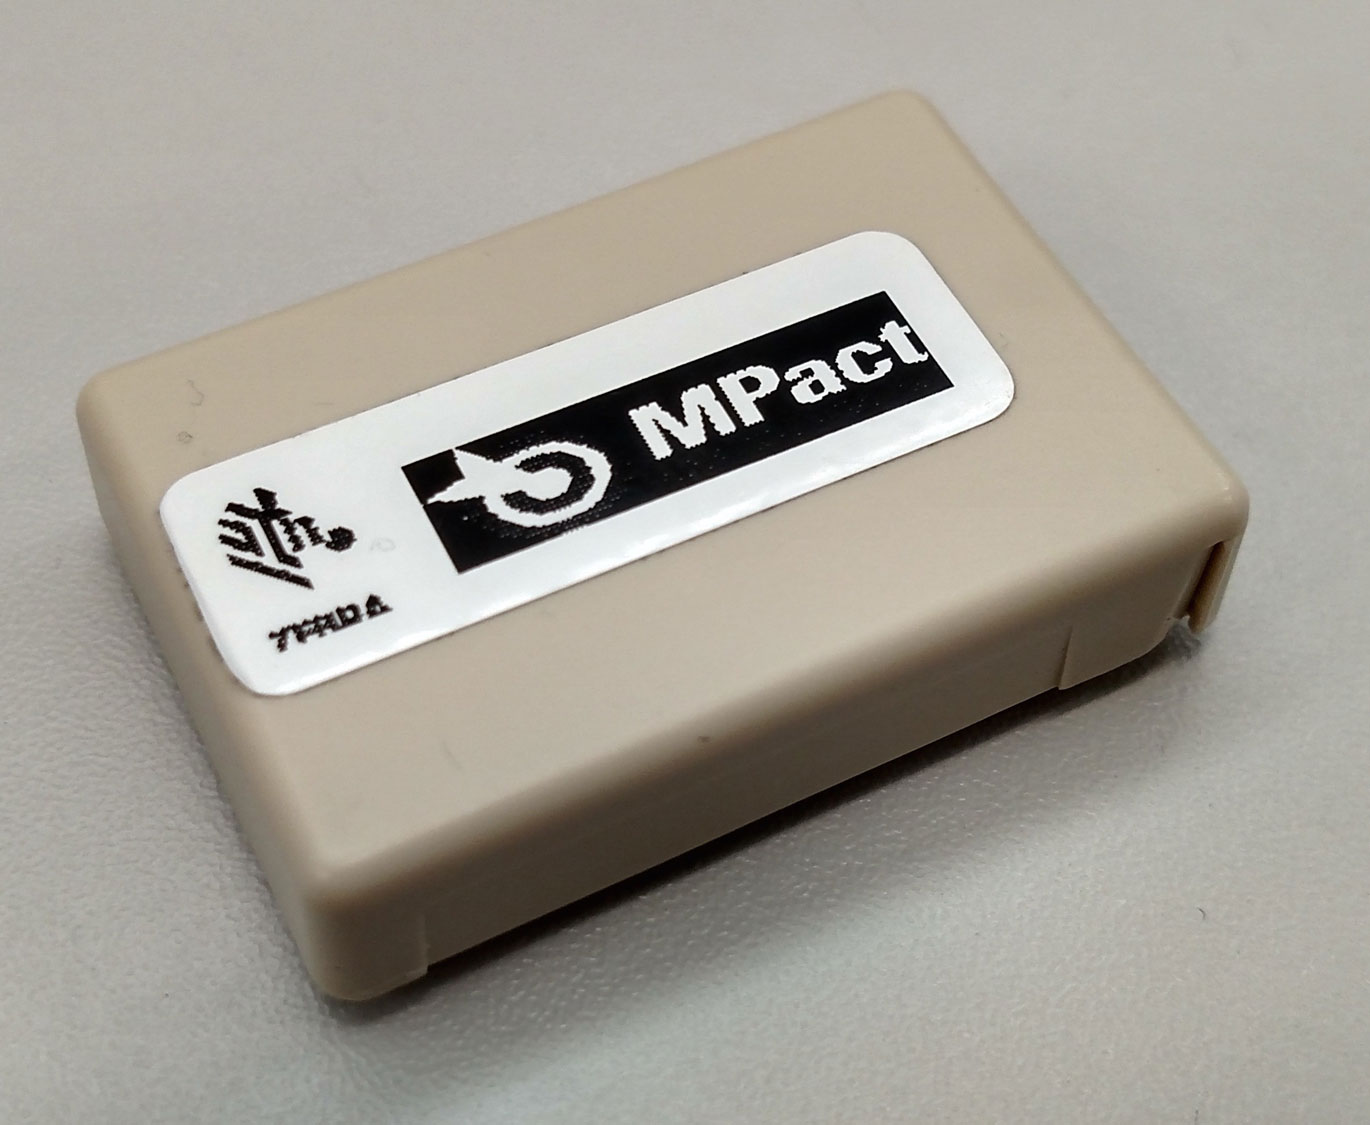
\includegraphics[width=0.6\textwidth]{img/beacon-mpact.jpg}
				\caption{Modelo de \textit{beacon} proprietário - MPact, da Zebra Technologies Corporation}
				\label{fig:beacon-mpact}
			}
		\end{figure}

Segundo \citeonline{teixeira-beacon}, os \textit{beacons} utilizam o \textit{BLE} para detectar um dispositivo próximo e transmitir seu identificador único e avisar que está ali presente. \citeonline{teixeira-beacon} também diz que os \textit{beacons} não são inteligentes, toda a interação deve depender do dispositivo que recebe a informação do identificador único.

Atualmente os usos de \textit{beacons} estão restritos a aplicativos em smartphones realizando a leitura e interagindo com o usuário, porém existem ainda diversas áreas a serem exploradas, e um bom exemplo são as casas inteligentes. Segundo \citeonline{grothaus-smarthomes}, a \textit{Apple} está apostando em um kit de desenvolvimento (\textit{HomeKit}) que permita aos desenvolvedores interagirem com \textit{smart devices} presentes no ambiente.

% ---

% ---
% Cronograma
% ---
\chapter{Cronograma}
% ---

A proposta é dividir o projeto em sete atividades: Pesquisa Bibliográfica, Estudo das Tecnologias, Análise e Planejamento, Definição da Estrutura, Implementação, Testes, Finalização do Projeto, conforme cronograma apresentado na Tabela~\ref{table:cronograma}.

\begin{table}[htb]
\IBGEtab{%
\ABNTEXchapterfont {
  \caption{Cronograma de Atividades Propostas}%
  \label{table:cronograma}
}
}{%
  \begin{tabular}{ccccccccc}
  \toprule
   Atividade & Jun & Jul & Ago & Set & Out & Nov & Dez & Jan \\
  \midrule \midrule
   Pesquisa Bibliográfica & X & X & X &   &   &   &   &   \\
  \midrule 
   Estudo das Tecnologias &  & X & X &   &   &   &   &   \\
  \midrule 
   Análise e Planejamento &   &   & X & X &   &   &   &   \\
  \midrule 
   Definição da Estrutura &   &   & X & X &   &   &   &   \\
  \midrule 
   Implementação &   &   &   & X & X & X &   &   \\
  \midrule 
   Testes &   &   &   &   & X & X & X &   \\
  \midrule 
   Finalização do Projeto &   &   &   &   &   &   & X & X \\
  \bottomrule
\end{tabular}%
}{%
  \fonte{Produzido pelo autor.}%
  }
\end{table}

% ---


% ---
% Conclusão
% ---
%\chapter{Conclusão}
% ---

%\lipsum[1]

% ---


% ----------------------------------------------------------------------------------------------------------------------------------






% ----------------------------------------------------------
% ELEMENTOS PÓS-TEXTUAIS
% ----------------------------------------------------------

% ----------------------------------------------------------

% ----------------------------------------------------------
% Referências bibliográficas
% ----------------------------------------------------------
\bibliography{referencias}

}
\end{document}